\documentclass{article}
\usepackage[utf8]{inputenc}
\usepackage[a4paper, total={6.5in, 9.5in}]{geometry}
\usepackage{float}
\usepackage{amsmath}
\usepackage{amssymb}
\usepackage{mathtools}
\usepackage{tensor}
\newcommand{\torseur}[7]{
\tensor[_{#1}]{\left\{ \begin{array}{cc}
    #2 & #5 \
    #3 & #6 \
    #4 & #7
\end{array} \right\}}{_{(\vec{x};\vec{y};\vec{z})}}
}
\usepackage{siunitx}
\sisetup{output-decimal-marker={,},group-minimum-digits=4,abbreviations}
\sisetup{inter-unit-product=\ensuremath{{}\cdot{}}}
\newcommand{\deftable}[2]{%
%\hline
\textbf{B.A.M.E}
\begin{table}[h]
    \centering
    \begin{tabular}{llp{130mm}}%
        %& unité/type & Explication \ \hline
        #1
    \end{tabular}
    \label{tab:#2_units}
\end{table}%
}
\newcommand{\deftablevar}[3]{%
    $#1$ & $\si{#2}$ & #3 \
}
\newcommand{\deftableobj}[3]{%
    $#1$ & \textit{#2} & #3 \
}
\newcommand{\bame}[1]{%
%\hline
\begin{table}[h]
    \centering
    \begin{tabular}{llllp{130mm}}%
        Nom & Vecteur & Direction & Sens & Norme \hline
        #1
    \end{tabular}
\end{table}%
}
\newcommand{\vect}[1]{\overrightarrow{#1}}

\title{Robot Sous-Marin}
\author{Ewen Le Bihan}
\date{2020-05-07}

\begin{document}

\maketitle

\section{}
\begin{equation*}
    \begin{split}
        v_{\max} &= \SI{3}{\meter\per\second} \\
        v_{\min} &= \SI{0}{\meter\per\second}
    \end{split}
\end{equation*}

Convertissons la vitesse maximale des marées à un coefficient de 45:

$$45\;\text{knots} = \SI{0.93}{\meter\per\second}$$



\section{}

Il possède une vitesse de pointe qui est le double de celle du ROV et est bien plus performant conçernant des fonctionnalités importantes comme le suivi de cap ou la giration

\section{}

\begin{table}[h]
    \centering
    \begin{tabular}{ll}
        FT121 & Stocker l'énergie\\
        FT141 & Cartographier la topologie des fonds marins \\
        FT142 & Acquérir un retour visuel\\
        FT17  & Communiquer les informations \\
    \end{tabular}
    \caption{Fonctions techniques manquantes}
    \label{tab:fonctions_techniques_manquantes}
\end{table}

\section{}

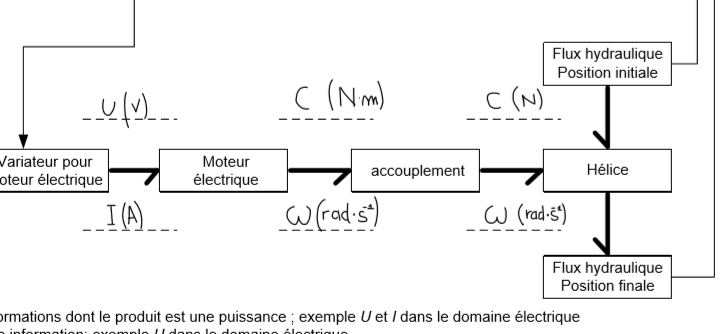
\includegraphics[width=\textwidth]{dr2.png}

\setcounter{section}{21}
\section{}

\begin{table}[h]
    \centering
    \begin{tabular}{ll}
        \texttt{PRE} & $\text{FA}_{16}$ \\
        \texttt{MID} & $\text{FF}_{16}$ \\
        \texttt{BID} & $\text{32}_{16}$
    \end{tabular}
    \caption{Valeurs des champs \texttt{PRE}, \texttt{MID} et \texttt{BID}}
    \label{tab:}
\end{table}

Taille du message: (en comptant $\texttt{TS}$): $37_{10} = 25_{16} = \texttt{LEN}$

Taille du message total:

$$ N_\text{octets} = \underbrace{1}_\texttt{PRE} + \underbrace{1}_\texttt{BID} + \underbrace{1}_\texttt{MID} + \underbrace{1}_\texttt{LEN} + \underbrace{37}_\texttt{DATA} + \underbrace{1}_\texttt{CS} = \text{réponse à la question de la vie} = 42$$

\section{}

Calculons la taille totale de la trame transmise $N_{\text{tot}} = 42 \cdot (8+2) = 420\;\text{bits}$

\begin{equation*}
    \begin{split}
        t_\text{sig} &= \frac{N_\text{tot}}{v_\text{trans}} \\
        &= \frac{\text{420 blaze it}}{2400} \\
        &= \SI{0.175}{\second}
    \end{split}
\end{equation*}

Sachant que le signal traverse l'eau, il faut prendre en compte un délai supplémentaire: 

\begin{equation*}
    \begin{split}
        t_\text{dly} &= d \div c_\text{son} \\
        &= 500 \div 1500 \\
        &= \SI{0.33}{\second}
    \end{split}
\end{equation*}

Donc, au total, le signal met une durée $t_\text{trans} = t_\text{sig} + t_\text{dly} = 0.175 + 0.33 = \SI{0.505}{\second}$.

\section{}

\begin{equation*}
    \begin{split}
        \frac{420}{0.505} &\approx 840\;\text{trames}
    \end{split}
\end{equation*}

\end{document}
